\newpage

\Large\textbf{Anhang}


%\begin{figure}
%    \centering
%    \includepdf[page= 1, scale=0.75]{content/MessdatenVXXX.pdf}
%\end{figure}
%
%\newpage
%
%\begin{figure}
%    \centering
%    \includepdf[page= 2, scale=0.75]{content/MessdatenVXXX.pdf}
%\end{figure}

\begin{figure}
    \centering
    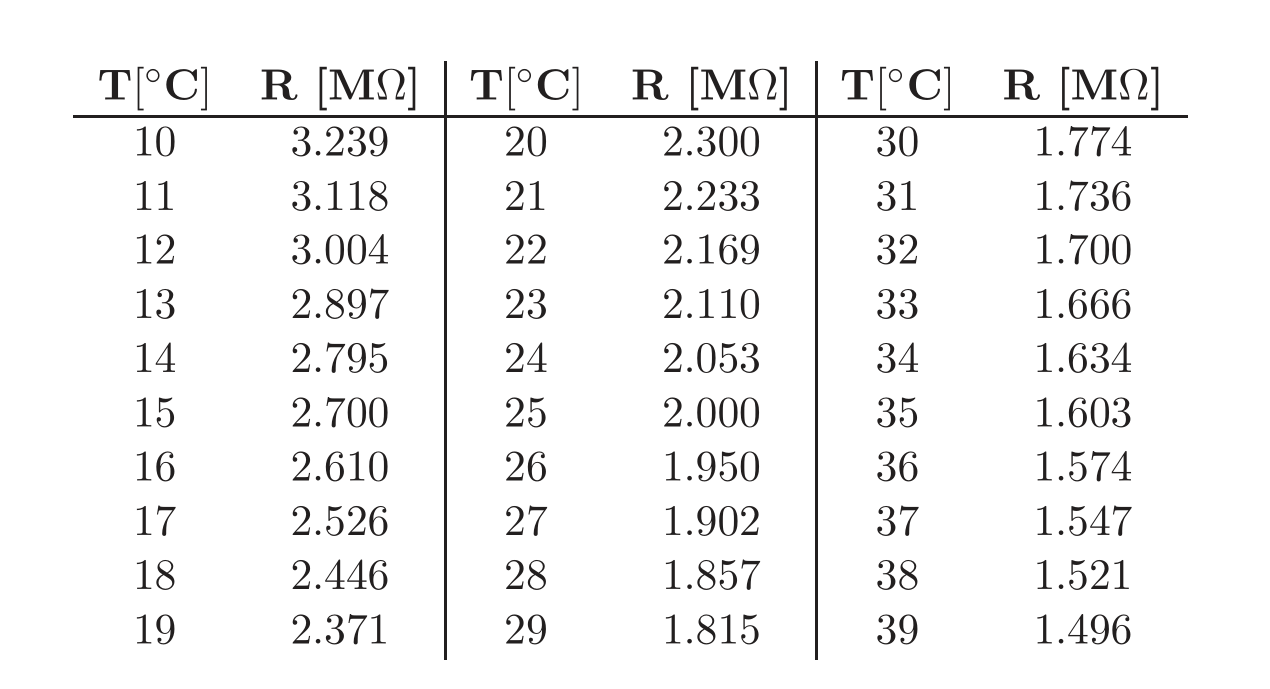
\includegraphics{content/Thermowiderstand.PNG}
    \caption{In dieser Grafik wird die Luftviskosität in Abhängigkeit von der Lufttemperatur angegeben. \cite{v503}}
    \label{fig:viskosität}
\end{figure}

\begin{figure}
    \centering
    \includegraphics{content/Thermowiderstando.PNG}
    \caption{In dieser Grafik wird die Lufttemperatur in Abhängigkeit des Thermowiderstandes dargestellt. \cite{v503}}
    \label{fig:Temperatur}
\end{figure}